\clearpage
\slidetitle{Réalisation Python}

\begin{slide}

	\begin{figure}[h]
		\centering
		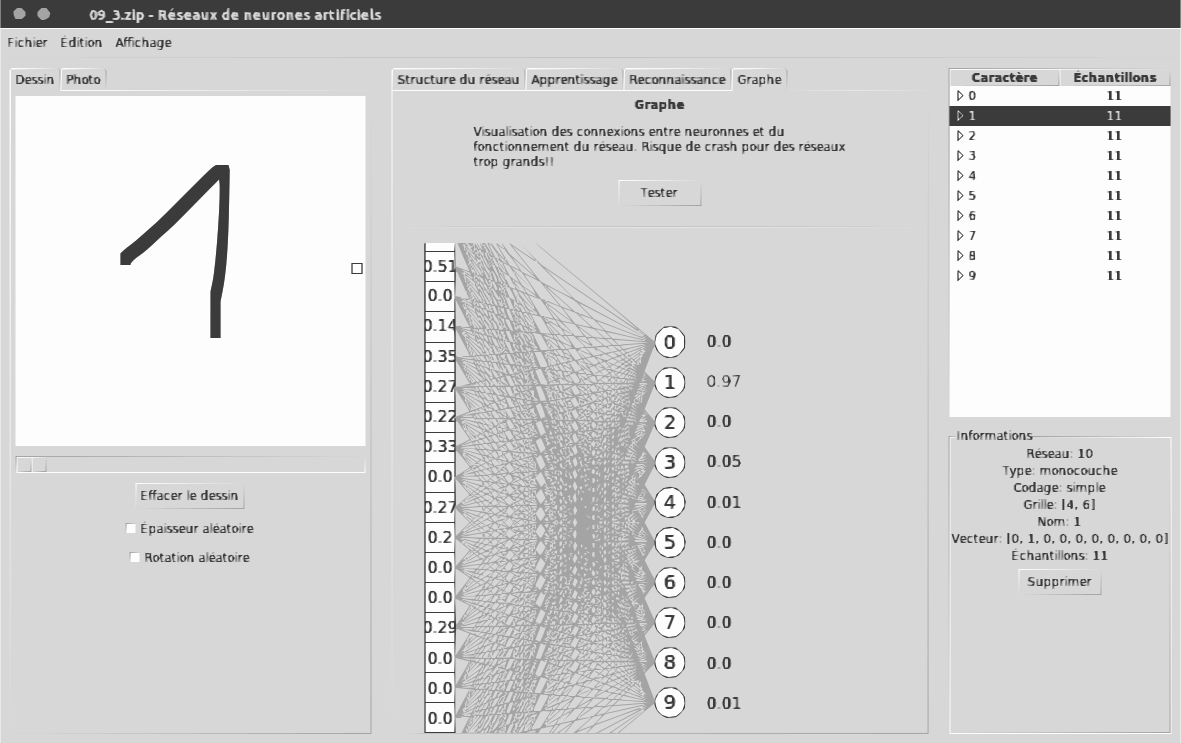
\includegraphics[width=\linewidth]{schemas/capture.png}
	\end{figure}

	\begin{itemize}
		\item Création d'une interface en Python permettant de créer un réseau et de l'entraîner à partir d'échantillons entrés à la souris.
	\end{itemize}

\end{slide}